%
% $Id: $
%
%
% Compilar a .pdf con LaTeX (pdflatex)
% Es necesario instalar Beamer (paquete latex-beamer en Debian)
%

%
% Gr�ficos:
% Los gr�ficos pueden suministrarse en PNG, JPG, TIF, PDF, MPS
% Los EPS deben convertirse a PDF (usar epstopdf)
%

\documentclass{beamer}
\usetheme{Warsaw}
%\usebackgroundtemplate{
\includegraphics[width=\paperwidth]{format/libresoft-bg.png}}
\usepackage[spanish]{babel}
\usepackage[latin1]{inputenc}
\usepackage{graphics}
\usepackage{amssymb} % Simbolos matematicos
\usepackage{url}

%\definecolor{libresoftgreen}{RGB}{162,190,43}
%\definecolor{libresoftblue}{RGB}{0,98,143}

%\setbeamercolor{titlelike}{bg=libresoftgreen}

%% Metadatos del PDF.
\hypersetup{
  pdftitle={Aprendizaje en Comunidad},
  pdfauthor={Agust�n Santos, Gregorio Robles},
  pdfcreator={GSyC/LibreSoft \\ Universidad Rey Juan Carlos},
  pdfproducer=PDFLaTeX,
  pdfsubject={Learning to code with Scratch. Community involvement.},
}
%%

\begin{document}

\title{Aprendizaje en Comunidad}
\subtitle{}
\institute{\{asantos,grex\}@gsyc.urjc.es \\
GSyC/Libresoft, Universidad Rey Juan Carlos}
\author{Agust�n Santos, Gregorio Robles}
\date{Curso de Verano UIMP, \#MECD\_UIMP15, Valencia, 10 de julio de 2015}

\frame{
\maketitle
\begin{center}

\includegraphics[width=2cm]{format/libresoft-logo}
\hspace{0.5cm}

\includegraphics[width=5cm]{format/gsyc-urjc}
\vspace{0.5cm}

\includegraphics[width=3cm]{format/emadrid.png}
\end{center}
}


% Si el titulo o el autor se quieren acortar para los pies de p�gina
% se pueden redefinir aqu�:
%\title{Titulo corto}
%\author{Autores abreviado}

%% LICENCIA DE REDISTRIBUCION DE LAS TRANSPAS
\frame{
~
\vspace{3cm}

\begin{flushright}

\includegraphics[width=2.2cm]{figs/by-sa}

{\tiny
(cc) 2015 Agust�n Santos M�ndez and Gregorio Robles\\
  Some rights reserved. This work licensed under Creative Commons \\
  Attribution-ShareAlike License. To view a copy of full license, see \\
  http://creativecommons.org/licenses/by-sa/3.0/ or write to \\
  Creative Commons, 559 Nathan Abbott Way, Stanford, \\
  California 94305, USA. \\
\ \\
Some of the figures have been taken from the Internet \\
Source, and author and licence if known, is specified. \\
For those images, \emph{fair use} applies.
}
\end{flushright}
}
%%

%\section{VII jornadas iTIC (\#iTIC15)}

%--------------------------------------------------------
\usebackgroundtemplate{
\includegraphics[width=11cm]{figs/hands.jpg}}

\begin{frame}
\frametitle{La importancia de la colaboraci�n}

Todos sabemos...
\begin{itemize}
  \item Que en equipo se llega m�s lejos
  \item Que en el mundo laboral, trabajar�n en equipo
\end{itemize}

Pero...
\begin{itemize}
  \item Ense�amos b�sicamente a construir desde cero
  \item Ense�amos a escribir c�digo, pero no a leer
\end{itemize}

\end{frame}

%--------------------------------------------------------
%\usebackgroundtemplate{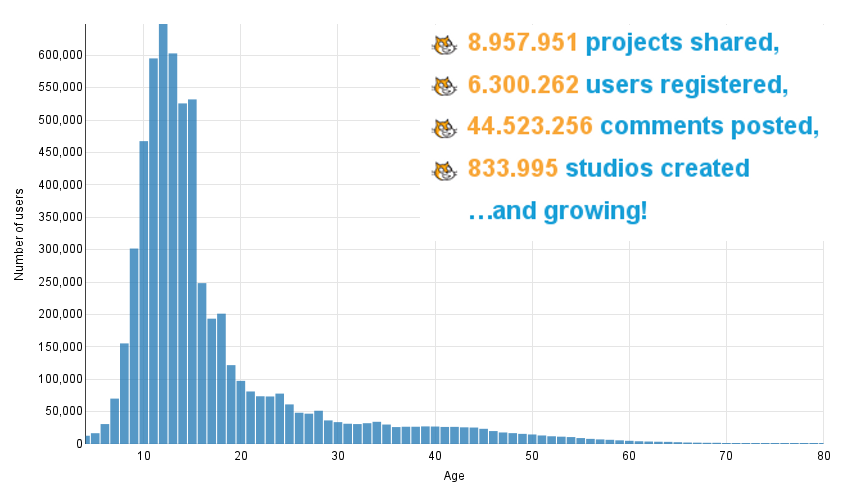
\includegraphics[width=18cm]{figs/stats.png}}
\usebackgroundtemplate{}

\begin{frame}
\frametitle{Colaborando que es gerundio}
\begin{columns}[T]
    \begin{column}{1\textwidth}
     \begin{block}{Tipos de colaboraci�n}
\begin{itemize}
  \item {\bf Impl�cita}: Toma mi c�digo y parte de ah� (la remezcla; implementada en la plataforma de Scratch)
  \item {\bf Expl�cita}: Trabajo colaborativo en equipo (por desgracia, a veces no es f�cil con la plataforma de Scratch)
\end{itemize}
    \end{block}
    \end{column}
  \end{columns}
\end{frame}

%--------------------------------------------------------
%\usebackgroundtemplate{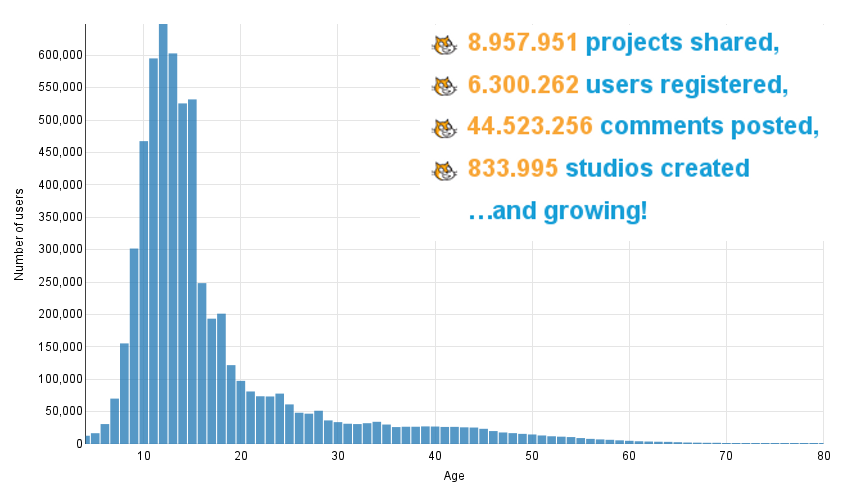
\includegraphics[width=18cm]{figs/stats.png}}

\begin{frame}
\frametitle{Remezclando proyectos existentes}

\begin{figure}[t!]
\begin{center}
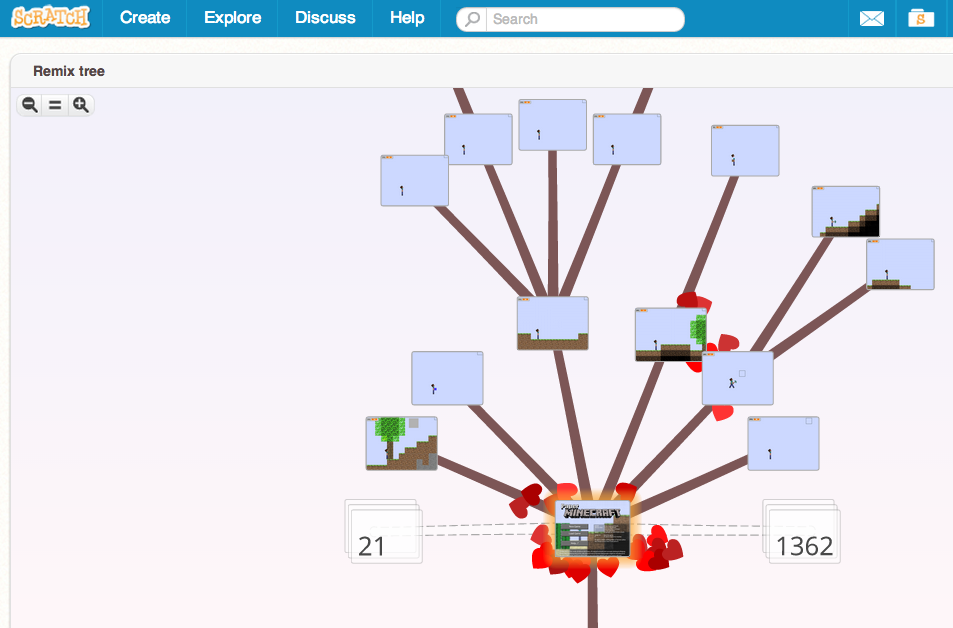
\includegraphics[width=10cm, height=6cm]{figs/remix.png}
\end{center}
\label{fig:remix}
\end{figure}
\begin{center}

\end{center}

\end{frame}

%--------------------------------------------------------
%\usebackgroundtemplate{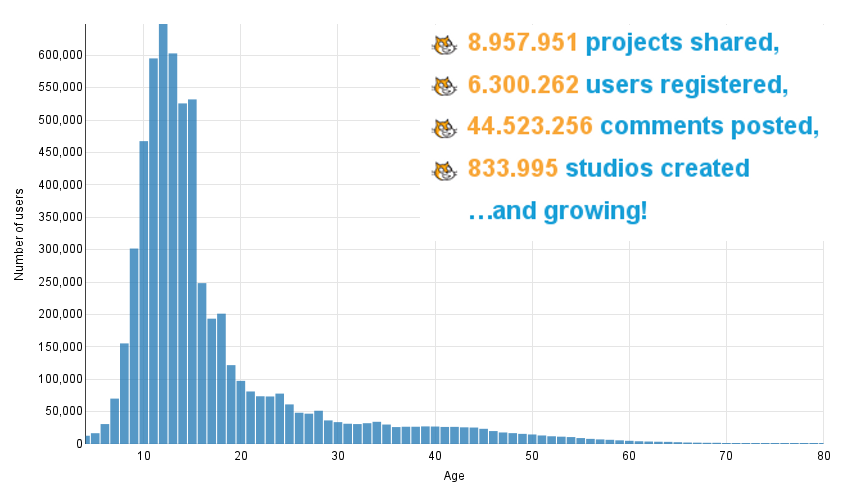
\includegraphics[width=18cm]{figs/stats.png}}
%
%\begin{frame}
%\frametitle{T�tulo Transpa}
%\begin{columns}[T]
%    \begin{column}{1\textwidth}
%     \begin{block}{Subt�tulo}
%\begin{itemize}
%  \item Punto 1
%\end{itemize}
%    \end{block}
%    \end{column}
%  \end{columns}
%\end{frame}


%--------------------------------------------------------
%\usebackgroundtemplate{\includegraphics[width=13cm]{figs/take-away.jpg}}
% background: http://2.bp.blogspot.com/-78Eh4TBpdtU/UPw7ULV73PI/AAAAAAAAHAE/6DQfvPNCo-Y/s1600/8723052-stylized-red-stamp-showing-the-term-take-away-all-on-white-background.jpg
%\usebackgroundtemplate{
\includegraphics[height=10cm,width=23cm]{figs/future.png}}
%
%\begin{frame}
%\frametitle{T�tulo}
%
%\begin{enumerate}
%  \item 
%\end{enumerate}
%\vspace{\baselineskip}
%\vspace{\baselineskip}
%\hfill{\Tiny Background picture: Simon Cunningham }
%
%\end{frame}



%--------------------------------------------------------
\usebackgroundtemplate{}

\frame{
\maketitle
\begin{center}

\includegraphics[width=2cm]{format/libresoft-logo}
\hspace{0.5cm}

\includegraphics[width=5cm]{format/gsyc-urjc}
\vspace{0.5cm}

\includegraphics[width=3cm]{format/emadrid.png}
\end{center}
}

\end{document}
